%% Creator: Inkscape inkscape 0.48.4, www.inkscape.org
%% PDF/EPS/PS + LaTeX output extension by Johan Engelen, 2010
%% Accompanies image file 'trajectory.pdf' (pdf, eps, ps)
%%
%% To include the image in your LaTeX document, write
%%   \input{<filename>.pdf_tex}
%%  instead of
%%   \includegraphics{<filename>.pdf}
%% To scale the image, write
%%   \def\svgwidth{<desired width>}
%%   \input{<filename>.pdf_tex}
%%  instead of
%%   \includegraphics[width=<desired width>]{<filename>.pdf}
%%
%% Images with a different path to the parent latex file can
%% be accessed with the `import' package (which may need to be
%% installed) using
%%   \usepackage{import}
%% in the preamble, and then including the image with
%%   \import{<path to file>}{<filename>.pdf_tex}
%% Alternatively, one can specify
%%   \graphicspath{{<path to file>/}}
%% 
%% For more information, please see info/svg-inkscape on CTAN:
%%   http://tug.ctan.org/tex-archive/info/svg-inkscape
%%
\begingroup%
  \makeatletter%
  \providecommand\color[2][]{%
    \errmessage{(Inkscape) Color is used for the text in Inkscape, but the package 'color.sty' is not loaded}%
    \renewcommand\color[2][]{}%
  }%
  \providecommand\transparent[1]{%
    \errmessage{(Inkscape) Transparency is used (non-zero) for the text in Inkscape, but the package 'transparent.sty' is not loaded}%
    \renewcommand\transparent[1]{}%
  }%
  \providecommand\rotatebox[2]{#2}%
  \ifx\svgwidth\undefined%
    \setlength{\unitlength}{488.56171875bp}%
    \ifx\svgscale\undefined%
      \relax%
    \else%
      \setlength{\unitlength}{\unitlength * \real{\svgscale}}%
    \fi%
  \else%
    \setlength{\unitlength}{\svgwidth}%
  \fi%
  \global\let\svgwidth\undefined%
  \global\let\svgscale\undefined%
  \makeatother%
  \begin{picture}(1,0.73685675)%
    \put(0,0){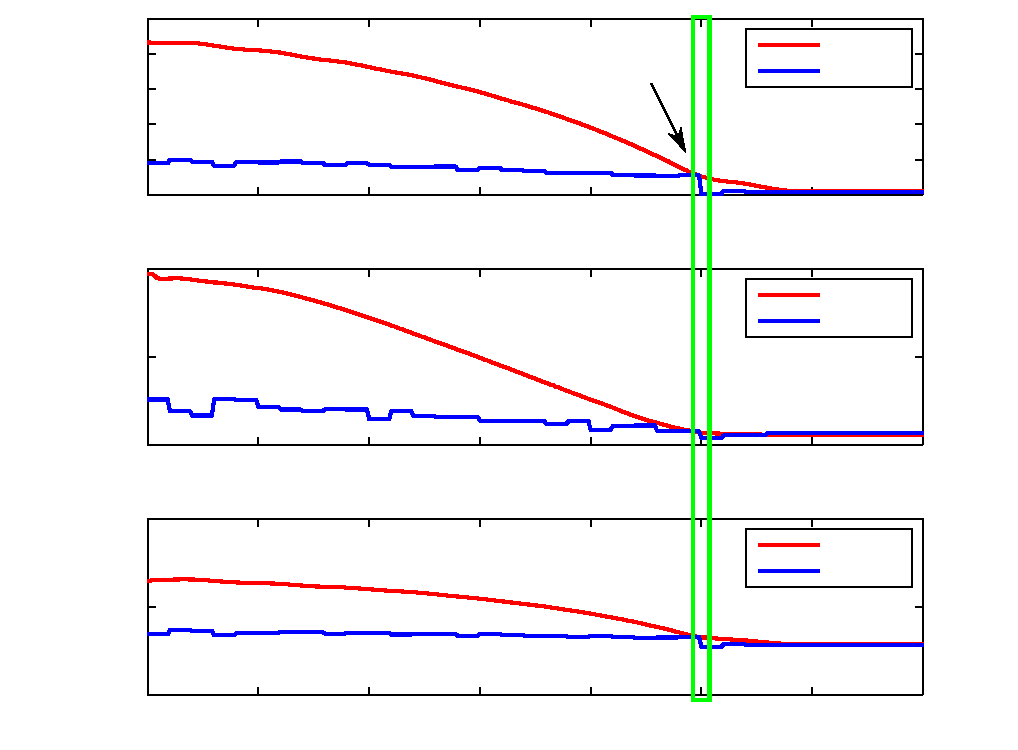
\includegraphics[width=\unitlength]{trajectory.pdf}}%
    \put(0.13965179,0.52057538){\makebox(0,0)[lb]{\smash{0}}}%
    \put(0.24830377,0.52057538){\makebox(0,0)[lb]{\smash{5}}}%
    \put(0.35149852,0.52057538){\makebox(0,0)[lb]{\smash{10}}}%
    \put(0.46031998,0.52057538){\makebox(0,0)[lb]{\smash{15}}}%
    \put(0.5689736,0.52057538){\makebox(0,0)[lb]{\smash{20}}}%
    \put(0.67779506,0.52057538){\makebox(0,0)[lb]{\smash{25}}}%
    \put(0.78661857,0.52057538){\makebox(0,0)[lb]{\smash{30}}}%
    \put(0.89544207,0.52057538){\makebox(0,0)[lb]{\smash{35}}}%
    \put(0.0990559,0.53780309){\makebox(0,0)[lb]{\smash{−0.9}}}%
    \put(0.0990559,0.5724288){\makebox(0,0)[lb]{\smash{−0.8}}}%
    \put(0.0990559,0.60722482){\makebox(0,0)[lb]{\smash{−0.7}}}%
    \put(0.0990559,0.64184972){\makebox(0,0)[lb]{\smash{−0.6}}}%
    \put(0.0990559,0.67630514){\makebox(0,0)[lb]{\smash{−0.5}}}%
    \put(0.52292005,0.4961846){\makebox(0,0)[lb]{\smash{t}}}%
    \put(0.81152228,0.68517444){\makebox(0,0)[lb]{\smash{xactual}}}%
    \put(0.81152228,0.65975943){\makebox(0,0)[lb]{\smash{xdesired}}}%
    \put(0.13965179,0.27495646){\makebox(0,0)[lb]{\smash{0}}}%
    \put(0.24830377,0.27495646){\makebox(0,0)[lb]{\smash{5}}}%
    \put(0.35149852,0.27495646){\makebox(0,0)[lb]{\smash{10}}}%
    \put(0.46031998,0.27495646){\makebox(0,0)[lb]{\smash{15}}}%
    \put(0.5689736,0.27495646){\makebox(0,0)[lb]{\smash{20}}}%
    \put(0.67779506,0.27495646){\makebox(0,0)[lb]{\smash{25}}}%
    \put(0.78661857,0.27495646){\makebox(0,0)[lb]{\smash{30}}}%
    \put(0.89544207,0.27495646){\makebox(0,0)[lb]{\smash{35}}}%
    \put(0.0990559,0.29218417){\makebox(0,0)[lb]{\smash{−0.1}}}%
    \put(0.08762807,0.37883279){\makebox(0,0)[lb]{\smash{−0.05}}}%
    \put(0.12805285,0.46531071){\makebox(0,0)[lb]{\smash{0}}}%
    \put(0.52292005,0.25056568){\makebox(0,0)[lb]{\smash{t}}}%
    \put(0.81152228,0.43955552){\makebox(0,0)[lb]{\smash{yactual}}}%
    \put(0.81152228,0.41414051){\makebox(0,0)[lb]{\smash{ydesired}}}%
    \put(0.13965179,0.02933754){\makebox(0,0)[lb]{\smash{0}}}%
    \put(0.24830377,0.02933754){\makebox(0,0)[lb]{\smash{5}}}%
    \put(0.35149852,0.02933754){\makebox(0,0)[lb]{\smash{10}}}%
    \put(0.46031998,0.02933754){\makebox(0,0)[lb]{\smash{15}}}%
    \put(0.5689736,0.02933754){\makebox(0,0)[lb]{\smash{20}}}%
    \put(0.67779506,0.02933754){\makebox(0,0)[lb]{\smash{25}}}%
    \put(0.78661857,0.02933754){\makebox(0,0)[lb]{\smash{30}}}%
    \put(0.89544207,0.02933754){\makebox(0,0)[lb]{\smash{35}}}%
    \put(0.0995676,0.04656525){\makebox(0,0)[lb]{\smash{0.89}}}%
    \put(0.08813977,0.13321388){\makebox(0,0)[lb]{\smash{0.895}}}%
    \put(0.11099625,0.21969179){\makebox(0,0)[lb]{\smash{0.9}}}%
    \put(0.52292005,0.00494676){\makebox(0,0)[lb]{\smash{t}}}%
    \put(0.81152228,0.1939366){\makebox(0,0)[lb]{\smash{zactual}}}%
    \put(0.81152228,0.16852159){\makebox(0,0)[lb]{\smash{zdesired}}}%
    \put(0.00442466,0.61404729){\color[rgb]{0,0,0}\makebox(0,0)[lb]{\smash{xtcp}}}%
    \put(-0.00048772,0.38480296){\color[rgb]{0,0,0}\makebox(0,0)[lb]{\smash{ytcp}}}%
    \put(-0.00048772,0.13918405){\color[rgb]{0,0,0}\makebox(0,0)[lb]{\smash{ztcp}}}%
    \put(0.45963838,0.68773296){\color[rgb]{0,0,0}\makebox(0,0)[lb]{\smash{switch
}}}%
  \end{picture}%
\endgroup%
